\clearpage
\thispagestyle{empty}

\begin{tikzpicture}[remember picture,overlay]

% Fond photographique
\node[
    anchor=center,
    opacity=0.30
] at (current page.center) {%
    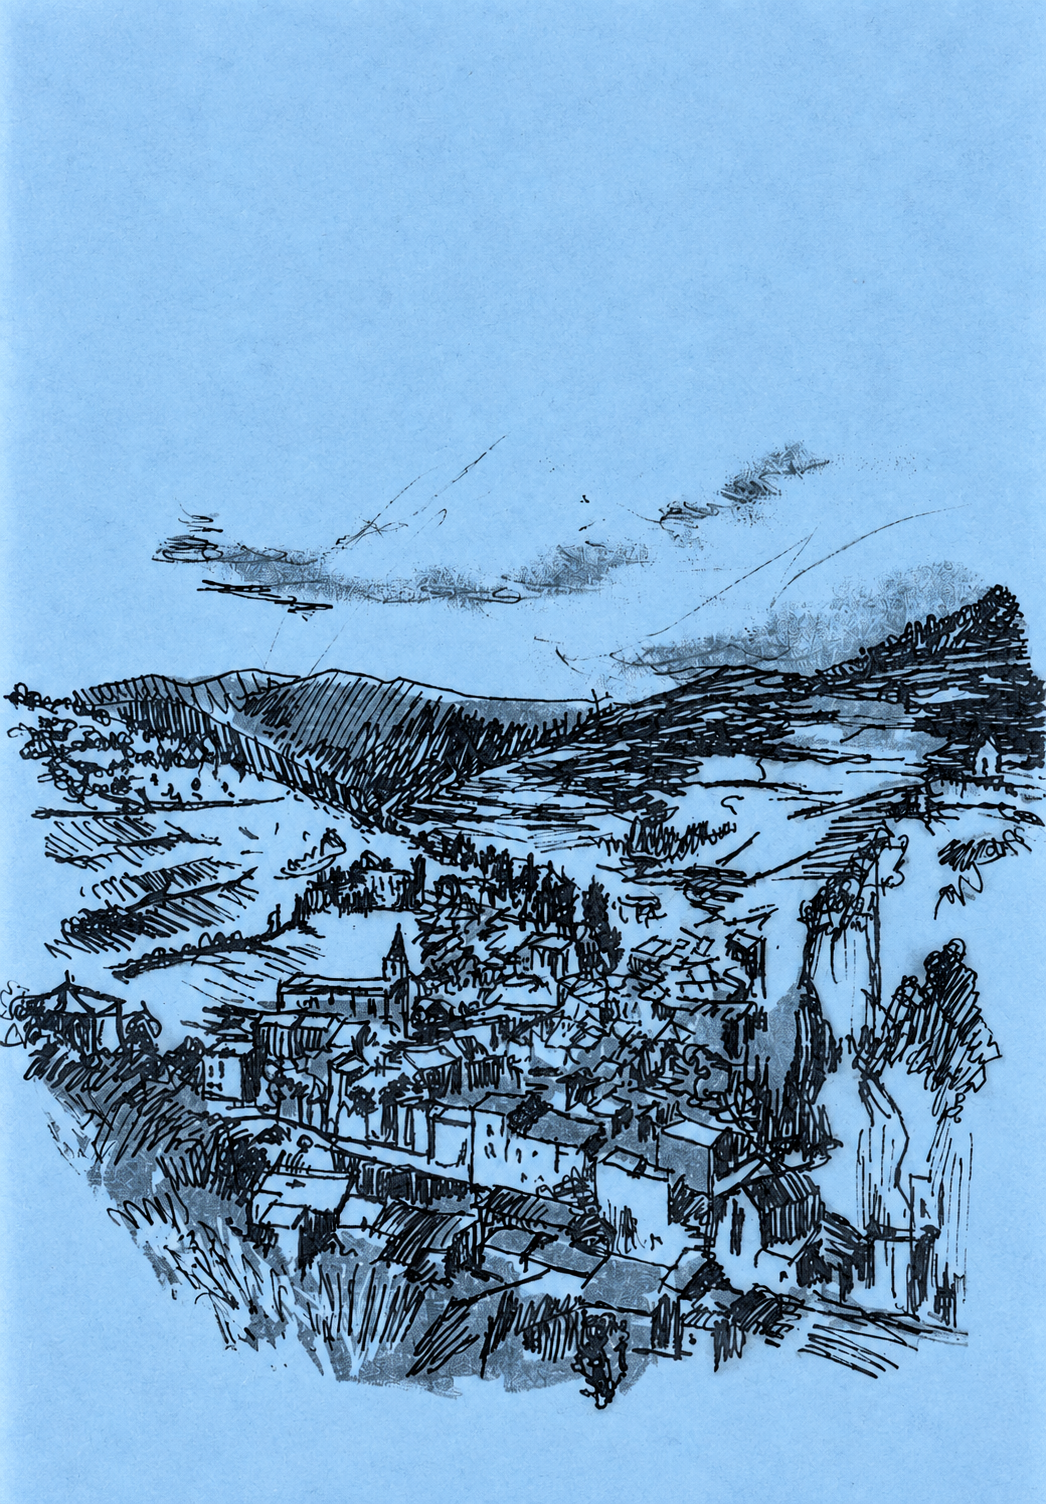
\includegraphics[
        width=\paperwidth,
        height=\paperheight,
        keepaspectratio=false
    ]{imgs/001}%
};

% Voile léger pour la lisibilité
\fill[
    white,
    opacity=0.55
]
(current page.south west)
rectangle
(current page.north east);

% Titre
\node[
    anchor=north,
    align=center,
    text width=0.82\paperwidth
]
at ([yshift=-3cm]current page.north)
{%
    {\fontsize{28}{34}\selectfont\bfseries MEYRUEIS}\\[0.3em]
    {\Large\itshape au fil du temps\ldots}
};

% Texte de présentation
\node[
    anchor=center,
    align=justify,
    text width=0.72\paperwidth,
    font=\small
]
at ([yshift=7cm]current page.center)
{%
    \textbf{De 1622 à 2000, Meyrueis au fil des souvenirs,
    des témoignages et des documents.}

    \medskip

    Cet ouvrage rassemble des récits, des archives,
    des photographies et des témoignages consacrés
    à Meyrueis et aux vallées qui l'entourent.

    \medskip

    De l'histoire protestante aux années de guerre,
    des anciennes activités économiques aux souvenirs
    de ceux qui ont vécu ici, ces pages font revivre
    des hommes, des lieux et des événements qui ont
    façonné la mémoire du pays.

\textbf{À propos de Paul Loupiac}

};

% --- À propos de Paul Loupiac ---

\node[
    anchor=north west,
    align=justify,
    text width=0.78\paperwidth,
    font=\small
]
at ([xshift=1.5cm,yshift=-15cm]current page.north west)
{%
    {\large\bfseries À propos de Paul Loupiac (1929-2021)}

    \medskip

    \textbf{Né à Lyon en février 1929}, Paul Loupiac était profondément
    attaché à ses racines meyrueisiennes. Son père, Franck Loupiac,
    s’était installé à Lyon après la cessation d’activité de la filature
    familiale du moulin d’Ayres.

    \medskip

    Pasteur dans plusieurs paroisses protestantes de la Drôme, de
    l’Ardèche et de la région parisienne, Paul Loupiac s’engagea ensuite
    pleinement auprès de \textit{l’Appel solidarité avec les enfants du
    monde}, dont il devint secrétaire général. Cette fonction l’amena à
    parcourir de nombreux pays, notamment en Afrique, au Salvador et à
    Madagascar.

    \medskip

    À la retraite, il s’installa à Montpellier avec son épouse Marianne,
    tout en continuant à retrouver, avec sa famille, la maison familiale
    du moulin d’Ayres. Très attaché à Meyrueis et à son histoire, il aimait
    évoquer ses souvenirs d’adolescent durant les années troublées de la
    Seconde Guerre mondiale, lorsqu’il vivait auprès de sa grand-mère.

    \medskip

    \textit{Ce livre est aussi le fruit de cet attachement : une mémoire
    patiemment rassemblée et transmise, pour que demeurent les histoires,
    les lieux et les hommes de Meyrueis.}
};

% Petite photo historique
\node[
    anchor=south east,
    inner sep=0pt
]
at ([xshift=-1.5cm,yshift=2cm]current page.south east)
{%
    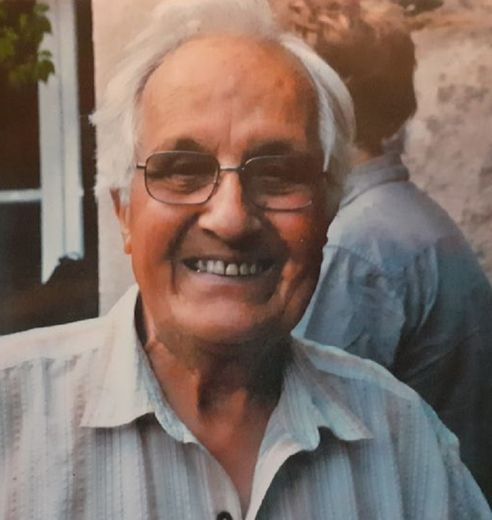
\includegraphics[
        width=4.5cm,
        keepaspectratio=false
    ]{imgs/paul_loupiac.jpg}%
};

% Crédit
\node[
    anchor=north east,
    font=\scriptsize\itshape
]
at ([xshift=-1.5cm,yshift=-0.2cm]current page.south east)
{Paul Loupiac};

\end{tikzpicture}

\clearpage
